\RequirePackage[orthodox]{nag}
\documentclass[11pt, reqno]{amsart}

\usepackage{amsmath}
	\numberwithin{equation}{section}
	\numberwithin{figure}{section}
\usepackage{amssymb}
\usepackage{amsthm}
\usepackage{verbatim}
\usepackage{fullpage}
\usepackage{color,fancyvrb}
\usepackage{microtype}
\usepackage{fancyhdr}
\usepackage{tikz}
\usetikzlibrary{automata,positioning}

%% DOCUMENT PARAMETERS
%% Adjust spacing, etc.
%% 
\linespread{1.3}
\setlength{\headheight}{15.2pt}
\setlength{\parskip}{6pt}
\setlength{\parindent}{0pt}
\setlength{\headsep}{12pt}
\setlength{\footskip}{15pt}

\pagestyle{fancy}
\thispagestyle{empty}

%% DECLARATIVE FORMATTING
%% Introduce new commands to standardize notation, etc.
%%
\newcommand{\mb}[1]{\mathbb{#1}}		% Math "blackboard" notation
\newcommand{\mc}[1]{\mathcal{#1}}		% Math "beautiful" notation
\newcommand{\mr}[1]{\mathrm{#1}}		% Math "Roman" notation

\newcommand{\R}{\mb{R}}
\newcommand{\N}{\mb{N}}

\newcommand{\theorem}[1]{
	\textit{Theorem.} #1}				% New theorem
\newcommand{\definition}[1]{
	\textit{Definition.} #1}			% New definition
\newcommand{\lemma}[1]{
	\textit{Lemma.} #1}				% New lemma
\newcommand{\corollary}[1]{
	\textit{Corollary.} #1}			% New corollary
\newcommand{\remark}[1]{
	\textit{Remark.} #1}				% New remark
%\newcommand{\em}[1]{{\emph #1}}
\newcommand{\question}[1]{\textit{#1}}	% Question
\newcommand{\term}[1]{\textbf{#1}}		% Highlighted term

\newcommand{\open}[1]{\left(#1\right)}	% Open interval
\newcommand{\closed}[1]{\left[#1\right]}	% Closed interval
\newcommand{\set}[1]{\left\{#1\right\}}	% Set
\newcommand{\discrete}[2]{
	\left\{#1..#2\right\}}			% Discrete interval, {1..4} -> {1,2,3,4}
\newcommand{\rmatrix}[1]{\left(\begin{matrix} #1 \end{matrix} \right)}
\newcommand{\smatrix}[1]{\left[\begin{matrix} #1 \end{matrix} \right]}

\newcommand{\sbs}{\subset}
\newcommand{\sps}{\supset}
\newcommand{\sbsq}{\subseteq}
\newcommand{\spsq}{\supseteq}

\newcommand{\length}[1]{\left|#1\right|}	% length of a word
\newcommand{\norm}[1]{\left\|#1\right\|}	% Norm
\newcommand{\dprod}[2]{#1 \cdot #2}		% Dot/inner product

\newcommand{\cartprod}[2]{#1 \times #2}	% Cartesian product
\newcommand{\inverse}[1]{#1^{-1}}		% Inverse function
\newcommand{\after}{\circ}				% Function composition
\newcommand{\restrict}[2]{#1\big|_{#2}}	% Function restriction

\newcommand{\Range}[1]{\mathcal{R}(#1)}	% Column space of a matrix
\newcommand{\Null}[1]{\mathcal{N}(#1)}	% Null space of a matrix
\newcommand{\transpose}[1]{#1^T}		% Transpose of a matrix or vector
\newcommand{\grad}[1]{\nabla #1}		% Gradient of a function
\newcommand{\diff}[1]{D#1}				% Differential of a function
\newcommand{\tangent}[1]{T_{#1}}		% Tangent space (to something) at a point
\newcommand{\opt}[1]{#1^*}				% Optimal vector or function

\newcommand{\rx}[1]{\textbf{#1}}  % Regular expression


\renewcommand{\perp}[1]{#1^{\perp}}		% "Perp" space
\renewcommand{\vec}[1]{#1}		% Alt. vector notation

\renewcommand{\implies}{\Rightarrow} 		% Long arrows suck
\renewcommand{\iff}{\Leftrightarrow} 		% Long arrows suck
\renewcommand{\epsilon}{\varepsilon} 		% I like varepsilon
\renewcommand{\qedsymbol}{$\blacksquare$}

\newcommand{\code}{\texttt}
\newcommand{\s}{\section}
\renewcommand{\ss}{\subsection}
\newcommand{\sss}{\subsubsection}

\pagestyle{myheadings}
\thispagestyle{empty}

\title{Automata}
\author{Course Notes}
\date{12 September 2015 -- 5 November 2015}

\begin{document}
\maketitle
\s*{Week 1: 12 September 2015 -- 18 September 2015}

\ss*{Homework Assignment 1.}

%\sss*{Question 1: Consider the above DFA. (I included the transition table as well.) Identify in the list below the string that this automaton accepts.}
\sss*{Question 2: The finite automaton from in Figure 1 accepts no word of length zero, no word of length one, and only two words of length two ($01$ and $10$). There is a fairly simple recurrence equation for the number $N(k)$ of words of length $k$ that this automaton accepts. Discover this recurrence and demonstrate your understanding by identifying the correct value of $N(k)$ for some particular $k$.}
\begin{figure}[hl]
\centering
\setlength\tabcolsep{10pt}
\begin{minipage}{0.48\textwidth}
\centering
\begin{tikzpicture}[shorten >=1pt,, >=latex, node distance=2cm,on grid,auto] 
   \node[state,initial] (q_0)   {$A$}; 
   \node[state] (q_1) [above right=of q_0] {$B$}; 
   \node[state] (q_2) [below right=of q_0] {$C$}; 
   \node[state,accepting](q_3) [below right=of q_1] {$D$};
    \path[->] 
    (q_0) edge  node {0} (q_1)
          edge  node [swap] {1} (q_2)
    (q_1) edge  node  {1} (q_3)
    (q_2) edge  node [swap] {0} (q_3) 
    (q_3) edge [swap] node {0} (q_0)
    (q_3) edge [swap, bend right=50] node {1} (q_1);
\end{tikzpicture}
%\caption{The finite automaton.}
\end{minipage}
%\hfill
\begin{minipage}{0.48\textwidth}
\centering
\begin{tabular}{r|c|r}
$\delta(q,x)$ & 0 & 1 \\
\hline
$\rhd$ A & B & C \\
       B & - & D \\
       C & D & - \\
$\ast$ D & A & B\\
\end{tabular}
%\caption{The transition table.}
\label{tab:ttable1}
\end{minipage}
\caption{The state diagram and transition table for the DFA in Questions 1 and 2.}
\end{figure}
\begin{proof}[Solution]
Suppose we are already at node $D$ (that is, we've made an acceptable string). How many strings of length $k$ could have gotten us here? Define $Q_n)$ to be the number of paths of length $n$ that terminate at $Q$. Initially we know that $A_0) = 1$, $B_0 = C_0 = D_0 = 0$. Now we also know the following recursion relations:
\[
A_n = D_{n - 1},\;
B_n = A_{n - 1} + D_{n - 1},\;
C_n = A_{n - 1},\;
D_n = B_{n - 1} + C_{n - 1}
\]
After some simplification this becomes the recurrence relation:
\[
D_n = D_{n - 2} + 2 D_{n - 3},\;
D_0 = D_1 = D_3 = 0,\;
D_2 = 2.\]
Now define $D(x) = \sum_{n \geq 0} D_n x^n$ to be the ordinary generating function of $D_n$. Taking our original relation, we multiply both sides by $x^n$ and sum over $n \geq 3$:
\[
\sum_{n \geq 3} D_n x^n = \sum_{n \geq 3} D_{n - 2} x^n + 2 \sum_{n \geq 3} D_{n - 3} x^n \quad \implies \quad
-2x^2 + \sum_{n \geq 0} D_n x^n = x^2 \sum_{j \geq 0} D_{j} x^j + 2 x^3 \sum_{k \geq 0} D_{k} x^k
\]
\[
-2x^2 + D(x) = x^2 D(x) + 2x^3 D(x) \quad \implies \quad
D(x) = \frac{2x^2}{1 - x^2 - 2x^3}
\]
Therefore $D_n$, the number of paths from $A$ to $D$ of length $n$, is just the coefficient of $x^n$ in the Taylor expansion of $D(x)$! By ``Wolfram's Theorem,'' we obtain the following values for $D_n$.
\begin{figure}[ht]
\setlength\tabcolsep{9pt}
\centering
\begin{tabular}{l || c | c | c | c | c | c | c | c | c | c | c | c | c | c | r}
$n$   &   0 &   1 &   2 &   3 &   4 &   5 &   6 &   7 &   8 &   9 &  10 &  11 &  12 &  13 &  14 \\
\hline
$D_n$ &   0 &   0 &   2 &   0 &   2 &   4 &   2 &   8 &  10 &  12 &  26 &  32 &  50 &  84 & 114 \\
\end{tabular}
\label{}
\caption{The first $15$ values of $D_n$.}
\end{figure}
\end{proof}

\sss*{Question 3: Given the above transition table (I also included the state diagram) of a simple DFA with start state $A$ and accepting state $B$, we want to show that this automaton accepts exactly those strings with an odd number of $1$'s, or more formally: $\delta(A, w) = B$ if and only if $w$ has an odd number of $1$'s. (Here, $\delta$ is the extended transition function of the automaton.)}
\begin{figure}[ht]
\centering
\setlength\tabcolsep{10pt}
\begin{minipage}{0.48\textwidth}
\centering
\begin{tabular}{r | c | r}
$\delta(q, x)$ & 0 & 1 \\
\hline
$\rhd$ A      & A & B \\
$\ast$ B      & B & A \\
\end{tabular}
\label{tab:ttable3}
\end{minipage}
\begin{minipage}{0.48\textwidth}
\centering
\begin{tikzpicture}[shorten >=1pt, >=latex, node distance=2cm,on grid,auto] 
   \node[state,initial]    (q_0)                {$A$}; 
   \node[state, accepting] (q_1) [right=of q_0] {$B$}; 
   \path[->] 
    (q_0) edge [loop above]   node {0} ()
          edge [bend left] node {1} (q_1)
    (q_1) edge [loop right]   node {0} ()
          edge [bend left] node {1} (q_0);
\end{tikzpicture}
\end{minipage}
\caption{} The state diagram and transition table for the DFA in Question 3.
\end{figure}

\begin{proof}
We proceed by induction on $\length{w}$, the length of $w$. For the base case, suppose $\length{w} = 0$. Then $w = \epsilon$, since the only word of length zero is the empty word. Now $w$ must have zero $1$'s as well, and by definition $\delta(A, \epsilon) = A$. Since zero is an even number, the statement holds for the base case.

Now assume that $\delta(A, x) = B$ if and only if $x$ has an odd number of $1$'s, for all $\length{x} \leq \length{w}$, and consider $w$. 
We have two cases: $w$ is of the form $w = x0$ or else it is of the form $w = x1$. 
Moreover, $x$ in each case may have either an even number or else an odd number of $1$'s. 
We need merely to exhaust all cases.
 
(1) Let $w = x0$ and $x$ has an even number of $1$'s. 
Then so does $w$, since we've appended no additional $1$'s. 
Now $\delta(A, w) = \delta(A, x0) = \delta(\delta(A, x), 0) = \delta(A, 0) = A$, by the inductive hypothesis and the transition table. 
Hence the statement holds for this case. 

(2) Let $w = x0$ and $x$ has an odd number of $1$'s. 
Then $w$ has an odd number of $1$'s, and $\delta(A, w) = \delta(A, x0) = \delta(\delta(A, x), 0) = \delta(B, 0) = B$. 
Again the statement holds. 

(3) Let $w = x1$ and $x$ has an even number of $1$'s. 
Then $w$ has an odd number of $1$'s since we just added an additional $1$. 
Now $\delta(A, w) = \delta(A, x1) = \delta(\delta(A, x), 1) = \delta(A, 1) = B$. 
Again the statement holds. 

(4) Let $w = x1$ and $x$ has an odd number of $1$'s. 
Then $w$ has an even number of $1$'s, and $\delta(A, w) = \delta(A, x1) = \delta(\delta(A, x), 1) = \delta(B, 1) = A$. 
Since the statement holds for this case as well as the other three, we have completed the proof.
\end{proof}
\newpage
\sss*{Question 4: Consider the non-deterministic finite automaton. Which strings does it accept?}
\begin{figure}[ht]
\begin{tikzpicture}[shorten >=1pt,node distance=2cm,on grid,auto] 
   \node[state,initial] (q_0)   {$A$}; 
   \node[state] (q_1) [right=of q_0] {$B$}; 
   \node[state, accepting] (q_2) [right=of q_1] {$C$}; 
   \path[->] 
    (q_0) edge [loop above] node {0} ()
          edge  node {1} (q_1)
    (q_1) edge  node {0} (q_2)
          edge [bend right=-45] node {0} (q_0)
    (q_2) edge [bend right=-85] node {1} (q_0)
          edge [bend right=-45] node {1} (q_1);
\end{tikzpicture}
\caption{The state diagram for the non-deterministic automaton in Question 4.}
\end{figure}
\begin{proof}[Solution]
We're given (e.g.) the following options: $0010010$, $00010111$, $01010011$, and $1011101$. In this case, the solution is trivial: we see that the only edge leading to the accepting state $C$ is labeled 0, and $C$ has no looped edges; hence the NFA cannot accept any strings that end in a 1. It remains to verify that $0010010$ is indeed an accepted string: indeed, the path $A \to A \to B \to A \to A \to B \to C$ corresponds with (part of) the output of $\delta_N(A, 0010010)$.
\end{proof}

\sss*{Question 5: Convert the NFA to a determinstic automaton. Which state is {\bf not} reachable from the start state \{A\}?}
\begin{figure}[ht]
\centering
\setlength\tabcolsep{10pt}
\begin{minipage}{0.48\textwidth}
\centering
\begin{tikzpicture}[shorten >=1pt, shorten <= 2pt, initial distance=.5cm, >=latex, node distance=2cm and 2.5cm, semithick, on grid, auto] 
   \node[state,initial]    (q_0)   {$A$}; 
   \node[state]            (q_1) [right=of q_0] {$B$}; 
   \node[state, accepting] (q_2) [above=of q_1] {$A,C$}; 
   \node[state]            (q_3) [right=of q_1] {$A, B$};
   \node[state]            (q_4) [below=of q_1] {};
   \path (q_0) edge [->, loop below]          node {0} ()
         (q_0) edge [->]                      node {1} (q_1)
         (q_1) edge [->]                      node  {0} (q_2)
         (q_1) edge [->]                      node  {1} (q_4)
         (q_2) edge [->, swap, bend right=10] node {1} (q_3)
         (q_2) edge [->, swap]                node {0} (q_0)
         (q_3) edge [->, swap, bend right=10] node {0} (q_2)
         (q_3) edge [->]                      node  {1} (q_1);
\end{tikzpicture}
\end{minipage}
%\hfill
\begin{minipage}{0.48\textwidth}
\centering
\begin{tabular}{r|c|r}
$\delta_D(\{q\},x)$ & 0 & 1 \\
\hline
$\rhd$ \{A\} & \{A\} & \{B\} \\
       \{B\} & \{A,C\} & \{ \} \\
$\ast$ \{A,C\} & \{A\} & \{A,B\} \\
       \{A,B\} & \{A, C\} &\{B\}\\
\end{tabular}
\end{minipage}
\caption{}The state diagram and transition table for the DFA constructed in Question 5.
\end{figure}
\begin{proof}[Solution]
We convert the NFA to a DFA using the subset construction. Notice that, in particular, the states $\{B, C\}$ and $\{A, B, C\}$ are not included, and therefore are not reachable from $\{A\}$.
\end{proof}
\newpage
\ss*{Challenge Problem 1.}
\sss*{Let $L$ be the language with alphabet $\{0, 1, 2\}$ consisting of strings that do not have any three consecutive $0$'s, any three consecutive $1$'s, or any three consecutive $2$'s. Prove that $L$ is a regular language (hint: design automata or regular expressions for some simpler languages and then use closure properties of regular languages to get $L$). Harder is to design a DFA $A$ for which the language is $L$ itself, but we encourage you try to design one as a second part of this exercise.}
\begin{proof}[Solution (closure)]
This solution exploits the fact that regular languages are closed under intersection. We first show that if $\Sigma = \{0, 1, 2\}$, then $L_a = \{x \in \Sigma^\ast : aaa \notin x\}$ is a regular language for any $a \in \Sigma$. %In fact, regular languages are closed under complements, so we need only show that $L_a^\prime = \{x \in \Sigma^\ast : aaa \in x\}$ is a regular language. The proof is trivial: $L_a^\prime$ is generated by the regular expression \rx{r}_a = $(abc)^\ast (aaa) (abc)^\ast$. This gives us insight into the DFAs for $L_a$ and $L_a^\prime$:
\begin{figure}[ht]
\centering
\begin{minipage}{0.48\textwidth}
\centering
\begin{tikzpicture}[shorten >=1pt, shorten <= 2pt, initial distance=.5cm, >=latex, node distance=2cm, semithick, on grid, auto] 
   \node[state] (q_0)                {$\diamond$}; 
   \node[state] (q_1) [right=of q_0] {}; 
   \node[state] (q_2) [right=of q_1] {}; 
   \node[state, accepting] (q_3) [right=of q_2] {};
   \path (q_0) edge [->, loop above]          node {b,c}   ()
         (q_0) edge [->]                      node {a}     (q_1)
         (q_1) edge [->]                      node {a}     (q_2)
         (q_1) edge [->, swap, bend right=45] node {b,c}   (q_0)
         (q_2) edge [->, bend left=30]        node {b,c}   (q_0)
         (q_2) edge [->]                      node {a}     (q_3)
         (q_3) edge [->, loop above]          node {}      (q_2);
\end{tikzpicture}
\end{minipage}
\begin{minipage}{0.48\textwidth}
\centering
\begin{tikzpicture}[shorten >=1pt, shorten <= 2pt, initial distance=.5cm, >=latex, node distance=2cm, semithick, on grid, auto] 
   \node[state, accepting] (q_0)                {$\diamond$}; 
   \node[state, accepting] (q_1) [right=of q_0] {}; 
   \node[state, accepting] (q_2) [right=of q_1] {}; 
   \node[state] (q_3) [right=of q_2] {};
   \path (q_0) edge [->, loop above]          node {b,c}   ()
         (q_0) edge [->]                      node {a}     (q_1)
         (q_1) edge [->]                      node {a}     (q_2)
         (q_1) edge [->, swap, bend right=45]       node {b,c}   (q_0)
         (q_2) edge [->, bend left=30]        node {b,c}   (q_0)
         (q_2) edge [->]                      node {a}     (q_3)
         (q_3) edge [->, loop above]          node {}      (q_2);
\end{tikzpicture}
\end{minipage}
\caption{The DFA state diagrams for $L_a^\prime$ (left) and $L_a$ (right).}
\end{figure}
Now, the choice of symbols is arbitrary, so the machine in Table 2 works for any choice of $a$ (respectively, $b$ and $c$) from $\Sigma$. Now we have three regular languages, $L_0$, $L_1$, $L_2$, each corresponding to the appropriate choice. Now we can take the intersection to get our new regular langugage, where none of $000$, $111$, or $222$ appears in a word\ldots except that this is exactly our original $L$! Hence $L$ is a regular language, and the problem is solved.\end{proof}
\begin{proof}[Solution (explicit)]
\begin{figure}[ht]
\centering
\setlength\tabcolsep{10pt}
\begin{tabular}{r | c | c | r}
$\delta(q, x)$   & 0   & 1   & 2   \\
\hline
$\ast$ $\rhd$    & x0  & x1  & x2  \\
$\ast$ x0        & x00 & x1  & x2  \\
$\ast$ x1        & x0  & x11 & x2  \\
$\ast$ x2        & x0  & x1  & x22 \\
$\ast$ x00       & err & x1  & x2  \\
$\ast$ x11       & x0  & err & x2  \\
$\ast$ x22       & x0  & x1  & err \\
       err       & err & err & err \\
\end{tabular}
\label{tab:ttable1c1}
\end{figure}
In this solution we construct an explicit DFA that accepts $L$, thus proving that $L$ is a regular language. We need the DFA to track whether it has seen three consecutive symbols---in which case it goes to an error state---but otherwise it can accept any word. This yields a relatively simple transition table. Unfortunately, the state diagram corresponding to this table is non-planar, so it cannot be easily drawn.
\end{proof} % 12 Sep -- 18 Sep
%\include{week2} % 19 Sep -- 25 Sep
%\include{week3} % 26 Sep --  2 Oct
%\include{week4} %  2 Oct --  8 Oct
%\include{week5} %  9 Oct -- 15 Oct
%\include{week6} % 16 Oct -- 22  Oct
%\include{week7} % 23 Oct -- 29  Oct
%\include{week8} % 30 Oct --  5  Nov

\end{document}